\newpage
\section{Aufgabe 1: a}

\subsection{Aufgabenstellung}
Machen Sie sich zunächst mit dem Befehl und den Parametern vertraut. Auch der Name Server, der von \texttt{nslookup} angesprochen wird, hat eine IP-Adresse. Wie lautet die Defaultadresse? Wie kann diese verändert werden? (1 Punkt)

\subsection{Vorbereitung}
Um diese Aufgabe lösen zu können, muss man sich mit dem Befehl \texttt{nslookup} auseinandersetzen und herausfinden wie man diesen konfiguriert. 

\subsection{Durchführung}
Die Default Adresse lautet \texttt{10.131.128.70} und kann mit einer \texttt{nslookup} Abfrage herausgefunden werden. Der erste Eintrag dort ist es.

\begin{figure}[H]
	\centering
	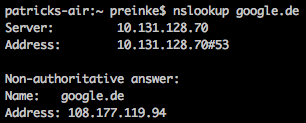
\includegraphics[width=0.4 \linewidth]{images/11}
	\caption{Ausführung von nslookup}
\end{figure}